\title{Chapter 3, Section 3. Exercises 1, 2 and 3}
\author{
	MTH 594, Prof. Mikael Vejdemo-Johansson \\
	Differential Geometry Independent Study \\
	\\
	Matthew Connelly \\
}
\date{\today}



\documentclass[12pt]{article}

\usepackage[top=.5in, bottom=.75in, left=1in, right=1in]{geometry}
\usepackage{amssymb}
\usepackage{amsmath}
\usepackage{graphicx}
\usepackage{subcaption}


\begin{document}
\maketitle

\section*{Exercise 3.3.1}

Show that the ellipse in Example 3.1.2 is convex.

\vspace{1cm}
\hrule
\vspace{1cm}
$\gamma(t) = (p \ cost, q \ sint)$ is our ellipse.

\begin{figure}[h!]
  \centering
      \begin{subfigure}[b]{0.5\linewidth}
    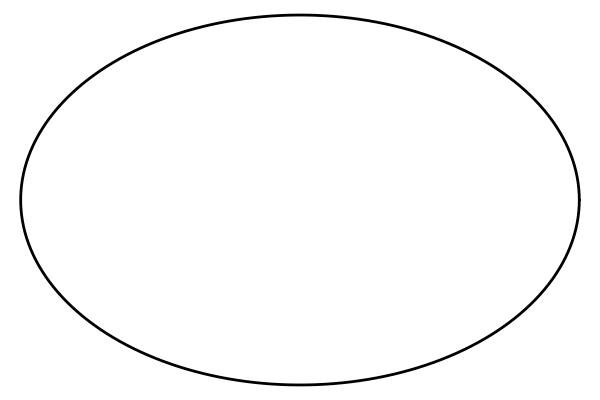
\includegraphics[width=\linewidth]{./assets/3-3-1/ellipse.png}
  \end{subfigure}
  \end{figure}
  
Our ellipse is convex if a straight line segment joining any two points of $Int(\gamma)$ is contained entirely within $Int(\gamma)$.\\

\indent
Because our ellipse is symmetrical about the $x$-axis, if it is convex above the $x$-axis, then it should also be convex below; meaning, there should be no surprises after $t = \pi$ (half of $\gamma$'s period).

\clearpage
We can then check $Int(\gamma)$ using a chord inscribed in the ellipse, between two diametrically opposed points:\\
\begin{figure}[h!]
  \centering
      \begin{subfigure}[b]{0.5\linewidth}
    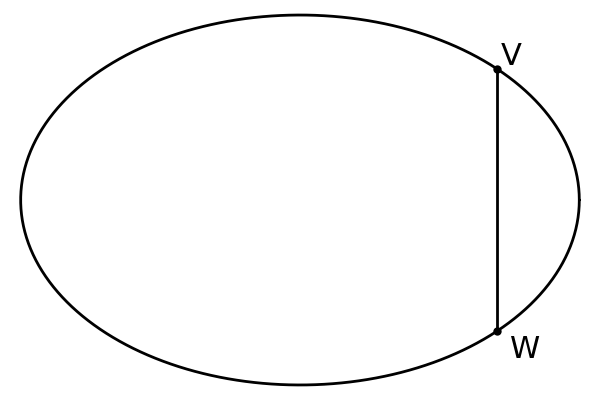
\includegraphics[width=\linewidth]{./assets/3-3-1/ellipse-vertical-chord.png}
  \end{subfigure}
  \end{figure}
  \\
  \indent
This chord can be written as:
$$
\overline{VW} = \gamma(-t) - \gamma(t)
$$
$$
\overline{VW} = y(-t) - y(t)
$$
$$
\overline{VW} = q \ (sin(-t)-sint)
$$
\indent
If we move this chord from right to left (or left to right), it will pass through all points of $Int(\gamma)$, and therefore intersect all possible line segments within $Int(\gamma)$ at least once.\\
\\
\indent
The distance between these two points then should not fluctuate if $\gamma$ is convex; if distance is increasing, it should continue to increase until achieving maximum distance, and if it is decreasing, it should continue to decrease until achieving zero distance, or else there will be a "valley" where a horizontal line may lie across $Ext(\gamma)$.

\begin{figure}[h!]
  \centering
      \begin{subfigure}[b]{0.5\linewidth}
    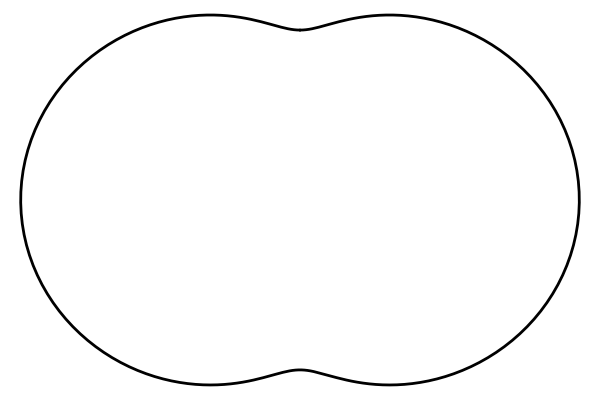
\includegraphics[width=\linewidth]{./assets/3-3-1/nephroid-degraded.png}
    \caption*{A degraded nephroid with a "valley" about its vertical axis of symmetry.}
  \end{subfigure}
  \end{figure}

\clearpage
The distance between $V$ and $W$ can be written as the following function:\\
$$
||\overline{VW}|| = D(t) = ( \ t, q \ (sin(-t) - sint) \ )
$$
Because of $\gamma$'s symmetry, we only need to evaluate $D(t)$ over $[0, \pi]$.
\begin{figure}[h!]
  \centering
      \begin{subfigure}[b]{0.7\linewidth}
    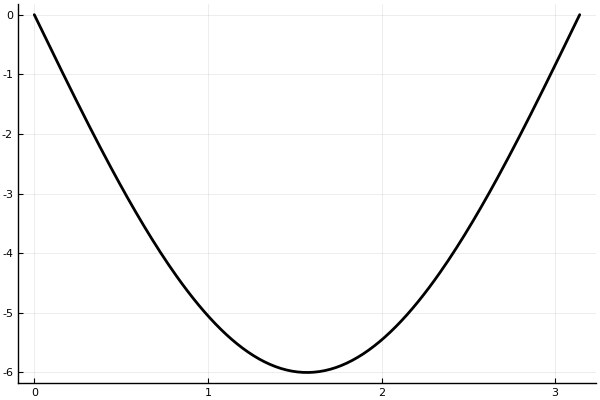
\includegraphics[width=\linewidth]{./assets/3-3-1/ellipse-chord-distance.png}
  \end{subfigure}
  \end{figure}

\end{document}
This is never printed